\documentclass[11pt]{amsart}          
\usepackage[a4paper,verbose]{geometry}
\geometry{top=3cm,bottom=3cm,left=3cm,right=3cm,textheight=595pt}
\setlength{\parskip}{0.3em}
% ==============================
% PACKAGES
% ==============================

\usepackage{amsfonts}
\usepackage{amssymb}  
\usepackage{amsthm} 
\usepackage{amsmath} 
\usepackage{caption}
\usepackage[inline]{enumitem}
\setlist{itemsep=0em, topsep=0em, parsep=0em}
\setlist[enumerate]{label=(\alph*)}
\usepackage{etoolbox}
\usepackage{stmaryrd} 
\usepackage[dvipsnames]{xcolor}
\usepackage[]{hyperref}
\hypersetup{
  colorlinks,
  linkcolor=blue,
  citecolor=blue,
  urlcolor=blue}
\usepackage{graphicx}
\graphicspath{{assets/}}
\usepackage{mathtools}

\usepackage{tikz-cd}
\usepackage{minted}
\usepackage{float}
\usetikzlibrary{
  matrix,
  arrows,
  shapes
}

\setcounter{tocdepth}{1} % Sets depth for table of contents. 

\newcommand{\rr}{{\mathbb{R}}}
\newcommand{\nn}{{\mathbb{N}}}
\newcommand{\iso}{\cong}
\newcommand{\too}{\longrightarrow}
\newcommand{\tto}{\rightrightarrows}
\newcommand{\To}[1]{\xrightarrow{#1}}
\newcommand{\Too}[1]{\To{\;\;#1\;\;}}
\newcommand{\from}{\leftarrow}
\newcommand{\From}[1]{\xleftarrow{#1}}
\newcommand{\Cat}[1]{\mathbf{#1}}
\newcommand{\cat}[1]{\mathcal{#1}}
\newtheorem*{remark}{Remark}
\renewcommand{\ss}{\subseteq}
\newcommand{\hask}[1]{\mintinline{Haskell}{#1}}
\newenvironment{haskell}
  {\VerbatimEnvironment
  	\begin{minted}[escapeinside=??, mathescape=true,frame=single, framesep=5pt, tabsize=1]{Haskell}}
  {\end{minted}}

\author{Bartosz Milewski}
\title{When is a functor representable?}

\begin{document}
\maketitle{}
Category theory is full of aha! moments. You open a book, read a sentence containing the words ``of course,'' or ``obviously,'' and have no idea what they are talking about. You start digging into it, go back to definitions of terms, draw a few pictures, and then you get it. It's a very satisfying feeling. 

I recently opened Max Kelly's book \emph{Basic Concepts of Enriched Category Theory} in the section about representable functors, in which he says that there is no simple criterion for deciding whether an enriched functor is representable. Then he remarks: 

``It is of course otherwise in the classical case $\cat V = \Cat{Set}$; there we have the comma category $1/F = el \,F$  of ``elements of F'', whose objects are pairs $(A, x)$ with $A \in \cat A$ and $x \in F A$; and $\alpha$ is invertible if and only if $(K, \eta)$ is initial in $el \, F$, so that $F$ is representable if and only if $el \, F$ has an initial object.''

If you understand this one-sentence explanation then you are a better person than me and you can stop reading right now. Otherwise, bear with me.

\section{Representable Functor}

Let's start with the definition of a representable functor. A functor $F$ from some category $\cat A$ to $\Cat{Set}$ is representable if there exists an object $K$ such that 
\[ \alpha \colon \cat A (K, -) \to F\]
is a natural isomorphism. In other words, for every object $A$ in $\cat A$ the set $F A$ is isomorphic to the hom-set $\cat A (K, A)$, and $\alpha$ is a family of bijections
\[\alpha_A \colon \cat{A} (K, A) \to F A\]

The \emph{unit} $\eta$ of the representation is the image of the identity morphism under $\alpha$
\[\eta = \alpha_K (id_K) \in F K\]

\section{Comma category}

A comma category is defined using three categories and two functors
\[ \cat B \xrightarrow{S} \cat C \xleftarrow{T} \cat A \]
 The name ``comma category'' is a historical accident. Modern notation for a comma category is either $S \downarrow T$ or $S / T$ (which is what Kelly uses). It is, essentially, a category of arrows in $\cat C$, whose sources come from the embedding of $\cat B$ using $S$, and targets come from  the embedding of $\cat A$ using $T$. So objects of $S / T$ are triples
 \[(B, A, f \colon S B \to T A)\]
 where $B$ is an object in $\cat B$, $A$ is an object in $\cat A$ and $f$ is a morphism in $\cat C$. 
 
 A morphism from $(B, A, f)$ to $(B', A', f')$ is a pair of morphisms $(h \colon B \to B', h' \colon A \to A')$ that makes the following diagram commute:
 
 \begin{figure}[H]
\centering
\begin{tikzcd}
S B
\arrow[r, "S h"]
\arrow[d, "f"]
& S B'
\arrow[d, "f'"]
\\
T A
\arrow[r, "T h'"]
& T A'
\end{tikzcd}
\end{figure}

This is a very general construction that can be specialized in many ways. For instance, you can take $\cat B$ to be the terminal single-object category. The functor $S$ then selects one object in $\cat C$. Furthermore, if $\cat C$ is  $\Cat{Set}$, you can specialize $S$ to pick the terminal set, the singleton $*$. In that case, the arrows in $S / T$ all have the singleton as the source. Such arrows pick individual elements in the set $T A$. 

If we call $1$ the functor that picks the singleton set $*$, and rename $T$ to $F$, we can say that the objects of the comma category $1 / F$ are pairs $(A, a)$ where $A$ is an object in $\cat A$ and $a$ is an element $a \in F A$.

A morphism from $(A, a)$ to $(A', a')$ is a morphism $h \colon A \to A'$ such that the following diagram commutes

\begin{figure}[H]
\centering
\begin{tikzcd}
& *
\arrow[ld, "a"']
\arrow[rd, "a'"]
\\
F A
\arrow[rr, "F h"]
&& F A'
\end{tikzcd}
\end{figure}
In other words, the lifted $h$ must map the point $a \in F A$ to the point $a' \in F A'$.

\section{Category of elements}

If you are intimately familiar with comma categories then the easiest way to describe the category of elements of a functor $F$ is to say that it's $1 / F$. For the rest of us, a more direct definition may be more intuitive. 

We start with a functor $F \colon \cat A \to \Cat{Set}$. The objects of $el \, F$ are pairs $(A, a \in F A)$, where $A$ is an object of $\cat A$. A morphism from $(A, a)$ to $(A', a')$ is a morphism $h \colon A \to A'$ such that $(F h) a = a'$. 

Let's dissect this definition a little. The category of elements explodes every object $A$ of $\cat A$ into as many separate objects of $el \, F$ as there are elements in the set $F A$. It's a giant disjoint union of sets $F A$ indexed by objects of $\cat A$. This is reflected in the coend notation
\[ el \, F = \int^{A: \cat A} F A \]

Every morphism $h$ of $\cat A$ explodes into as many morphisms of $el \, F$ as there are elements in the domain of $F h$. So a morphism is $el \, F$ is uniquely determined by a pair 
\[(h \colon \cat A (A, A'), a \in F A)\]
The domain of this morphism is $(A, a)$ and the codomain is $(A', (F h) a)$.

Moreover, for a fixed pair $(A, a)$, we get a natural transformation

\[ \phi^{(A, a)} \colon \cat A (A, -) \to F\]
whose component at $A'$ is implemented by lifting $h \in \cat A (A, A')$ and applying it to $a$
\[ \phi^{(A, a)}_{A'} h = (F h) a\]
This mapping is natural in $A'$. To show this, suppose that we have a morphism $f \colon A' \to A''$. The naturality square is

 \begin{figure}[H]
\centering
\begin{tikzcd}
\cat A (A, A')
\arrow[r, "f \circ -"]
\arrow[d, "\phi_{A'}"]
& \cat A (A, A'')
\arrow[d, "\phi_{A''}"]
\\
F A'
\arrow[r, "F f"]
& F A''
\end{tikzcd}
\end{figure}
Indeed, acting on $h \in \cat A (A, A')$, the composition with $f$ produces $f \circ h$ and then $\phi_{A''}$  produces $ (F (f \circ h)) a$. By functoriality, this is equal to $(F f) ((F h) a)$. The other path produces first $(F h) a$ and then acts on it with $F f$. 


Notice that, in order to show that $F$ is representable, all we have to do is to find a pair $(A, a)$ for which $\phi^{(A, a)}$ is an isomorphism. In other words, every component of $\phi^{(A, a)}$ must be a bijection of sets. 

There are two ways in which this condition may break down. First, it's possible that two morphisms $h$ and $h'$ from the same hom-set $\cat A (A, A')$ produce the same element $a'$ in $F A'$. In other words, it's possible to have two different morphisms in $el \, F$ from $(A, a)$ to $(A', a')$. 

The other way of not being bijective is if there is an element $a'$ in $A'$ that is not covered by our mapping. In other words, there may be no such $h$ in $\cat A (A, A')$ for which $(F h) a$ is equal to $a'$. That would mean that there is no morphism in $el \, F$ from $(A, a)$ to $(A', a')$.

What we need is to have exactly one morphism from $(A, a)$ to $(A', a')$. That is only possible if $(A, a)$ is the initial object.

\section{Initial object in the category of elements}

Suppose that there is an initial object in the category of elements $el \, F$. It's a pair $(K, \eta)$, where $\eta$ is an element of $F K$. There is a unique morphism from it to any other object $(A, a)$ of $el \, F$. Such a morphism is a morphism $h \in \cat A (K, A)$, such that $F h$ maps $\eta$ to $a$. 

Let's dissect this statement. For every $h$ we can produce an element $a$ of $F A$
\[ a = (F h) \eta\]
That gives us a mapping
\[\alpha_A \colon \cat A (K, A) \to F A\]
Initiality of $(K, \eta)$ means that this mapping is a bijection. We can reach every $a \in F A$ and every $h$ maps $\eta$ to a different $a$. 

\begin{figure}[H]
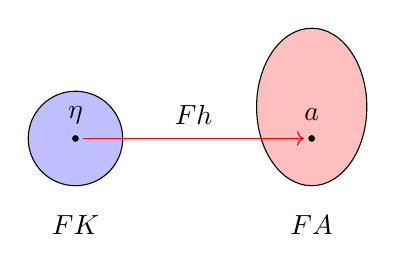
\begin{tikzpicture}
         \draw (-1.5,0)[fill=blue!25!white] ellipse (0.6 and 0.6);
         \draw ( 1.5,0.4)[fill=red!25!white] ellipse (0.7 and 1);
        \node at (-1.5, 0.3) { $\eta$ };
        \node at ( 1.5, 0.3) { $a$ };
        \filldraw (1.5, 0.0) circle (1pt);
        \filldraw (-1.5, 0.0) circle (1pt);
	\draw[->, red] (-1.4, -0.0) -- (1.4, 0.0);
        \node at (0, 0.3) { $F h$ };
        \node at (-1.5, -1.1) { $F K$ };
        \node at (1.5, -1.1) { $F A$ };
\end{tikzpicture}
\end{figure}
This proves that $F$ is representable if and only if $el \,F$ has an initial object. So it was obvious after all!

\end{document}


